\documentclass[10pt]{gulartcl}
\usepackage{../exstyle}

\title{Esercizio settimanale n. 1}
\author{Guglielmo Bordin}
\date{\today}

% defining hexagon macro
\newcommand{\hexagon}{%
    \newdimen\side
    \side = 2cm
    \draw[densely dashed] (0:\side) \foreach \angle in {60, 120, ..., 360}{
        -- (\angle:\side)
    };
    \foreach \i/\pos in
        {1/right, 2/above, 3/above, 4/left, 5/below, 6/below}{
        \node[inner sep=1pt, circle, draw, fill, label={\pos:{$q_{\i}$}}]
            at ({60 * (\i - 1)}:\side) {};
    };}

\begin{document}
\maketitle

\noindent
Sei cariche $q_{n} = n q$, con $n = 1, 2, \dots, 6$ e $q = \qty{1}{pC}$,
sono disposte ai vertici di un esagono regolare di lato $a = \qty{1}{cm}$
come in figura. Calcolare le componenti lungo gli assi $x$ e $y$ del campo
elettrico al centro dell’esagono.

\bigbreak
\begin{center}
\begin{tikzpicture}
    \hexagon
    \draw[-latex] (2.5, 1) -- ++(1, 0) node[near end, below] {$x$};
    \draw[-latex] (2.5, 1) -- ++(0, 1) node[near end, left] {$y$};
    \coordinate (A) at ($(240:\side) + (0, 0.2)$);
    \coordinate (B) at ($(300:\side) + (0, 0.2)$);
    \draw[latex-latex] (A) -- (B) node[midway, above] {$a$};
\end{tikzpicture}
\end{center}

\begin{solution}
La carica $q_n$ produce un campo elettrico che al centro dell’esagono vale,
in modulo,
\begin{equation}
    E_n = \frac{n q}{4 \pi \epsilon_0 a^2}.
\end{equation}
Le direzioni sono quelle indicate in figura~\ref{fig:six-vectors}, in
grigio. Notiamo che sommando lungo le rette congiungenti le coppie di
vertici opposti si ottengono tre campi, che denotiamo $\vec{E}_{1, 4}$,
$\vec{E}_{2, 5}$ ed $\vec{E}_{3, 6}$, di modulo
\begin{equation}
    E_{n, n + 3} = E_{n + 3} - E_{n} = \frac{(n + 3) q}{4 \pi \epsilon_0
    a^{2}} - \frac{n q}{4 \pi \epsilon_0 a^{2}} = \frac{3 q}{4 \pi
\epsilon_0 a^2}.
\end{equation}

\begin{figure}
    \centering
    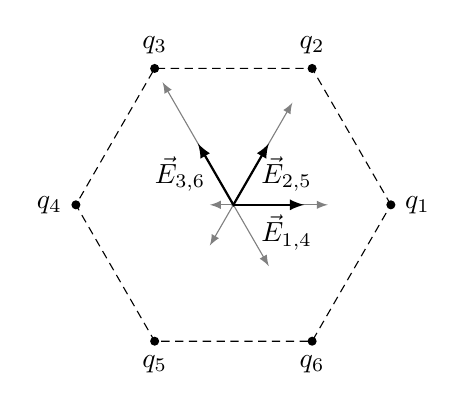
\begin{tikzpicture}
        \hexagon
        \filldraw (0, 0) circle (0.5pt);
        \foreach \i in {1, 2, ..., 6}{
            \draw[-latex, gray] (0, 0) -- ({60 * (\i - 1) + 180}:{\i * 0.3});
        }
        \draw[-latex, thick] (0, 0) -- (0:0.9) node[near end, below]
            {$\vec{E}_{1, 4}$};
        \draw[-latex, thick] (0, 0) -- (60:0.9) node[pos=0.5, right]
            {$\vec{E}_{2, 5}$};
        \draw[-latex, thick] (0, 0) -- (120:0.9) node[pos=0.5, left]
            {$\vec{E}_{3, 6}$};
    \end{tikzpicture}
    \caption{in grigio i campi prodotti dalle singole cariche, e in nero le
    somme lungo le rette congiungenti i vertici opposti.}
    \label{fig:six-vectors}
\end{figure}

Guardando il disegno vediamo che la componente $x$ del campo risultante
$\vec{E}$ è uguale a $\vec{E}_{1, 4}$, poiché nella somma degli altri due
vettori le componenti orizzontali si cancellano per simmetria.  La
componente $y$ di $\vec{E}$ sarà invece data dalla somma delle proiezioni
di $\vec{E}_{2, 5}$ ed $\vec{E}_{3, 6}$ lungo l’asse $y$, ossia
\begin{equation}
    E_{y} = E_{2, 5} \cos\left(\frac{\pi}{6}\right) + E_{3, 6}
    \cos\left(\frac{\pi}{6}\right) = 2 \frac{3q}{4 \pi \epsilon_0 a^{2}}
    \frac{\sqrt{3}}{2} = \frac{3 \sqrt{3} q}{4 \pi \epsilon_{0} a^{2}}.
\end{equation}

In definitiva avremo quindi
\begin{equation}
    \vec{E} = \frac{3 q}{4 \pi \epsilon_0 a^{2}} \uvec{x} + \frac{3
    \sqrt{3} q}{4 \pi \epsilon_0 a^{2}} \uvec{y},
\end{equation}
e sostituendo i valori numerici,
\begin{equation}
    E_x = \qty{270}{N/C}, \quad E_y = \qty{470}{N/C}.
\end{equation}
Il modulo di $\vec{E}$ è invece pari a
\begin{equation}
    E = \sqrt{\smash[b]{E_x^{2} + E_y^{2}}} = \frac{3 q}{4 \pi \epsilon_0
    a^2} \sqrt{\smash[b]{1 + (\sqrt{3})^2}} = \frac{3 q}{2 \pi \epsilon_0
    a^{2}} = \qty{540}{N/C}.
\end{equation}
La direzione è quella di $\vec{E}_{2, 5}$: lo si può capire
ragionando sulla somma di $\vec{E}_{1, 4}$ ed $\vec{E}_{3, 6}$. Le
componenti perpendicolari alla direzione di $\vec{E}_{2, 5}$ si cancellano
per simmetria, e rimangono solo le componenti parallele.
\end{solution}
\end{document}
